\documentclass{beamer}
\usepackage{minted}
\usepackage{hyperref}
\usepackage[style=numeric]{biblatex}
\usepackage{subfig}
\addbibresource{../main.bib}
\usepackage{xcolor}
\usetheme{metropolis}
\definecolor{cvutblue}{RGB}{1,44,86}

\newcommand{\reffig}[1]{Fig.~\ref{#1}}
\newcommand{\reflst}[1]{Lst.~\ref{#1}}
\newcommand{\refalg}[1]{Alg.~\ref{#1}}
\newcommand{\refsec}[1]{Sec.~\ref{#1}}
\newcommand{\reftab}[1]{Table~\ref{#1}}
\newcommand{\refeq}[1]{\eqref{#1}}

\setbeamercolor{palette primary}{bg=cvutblue,fg=white}
\title{Analysis of an influnce of a modulated light source frequency
and distance on an event-based camera response}

\date{23.1.2025}
\author{Jakub Pelc}

\institute{Faculty of Electrical Engineering, Czech Technical University in Prague}
\begin{document}
	\maketitle

	\begin{frame}{Goals of this bachelor thesis}
	Estimate the pose of a UAV marked with modulated LED lights.
	\end{frame}

	\begin{frame}{Distance influence}


	\end{frame}

	\begin{frame}{Event-based camera response}
		%distance frequency rotation influence
	\end{frame}

	\begin{frame}[allowframebreaks]{Experimental validation of the inverse square law}

		\begin{equation}
			\text{intensity} \propto \frac{1}{\text{distance}^2}
		\end{equation}

		\begin{figure}
			\centering
			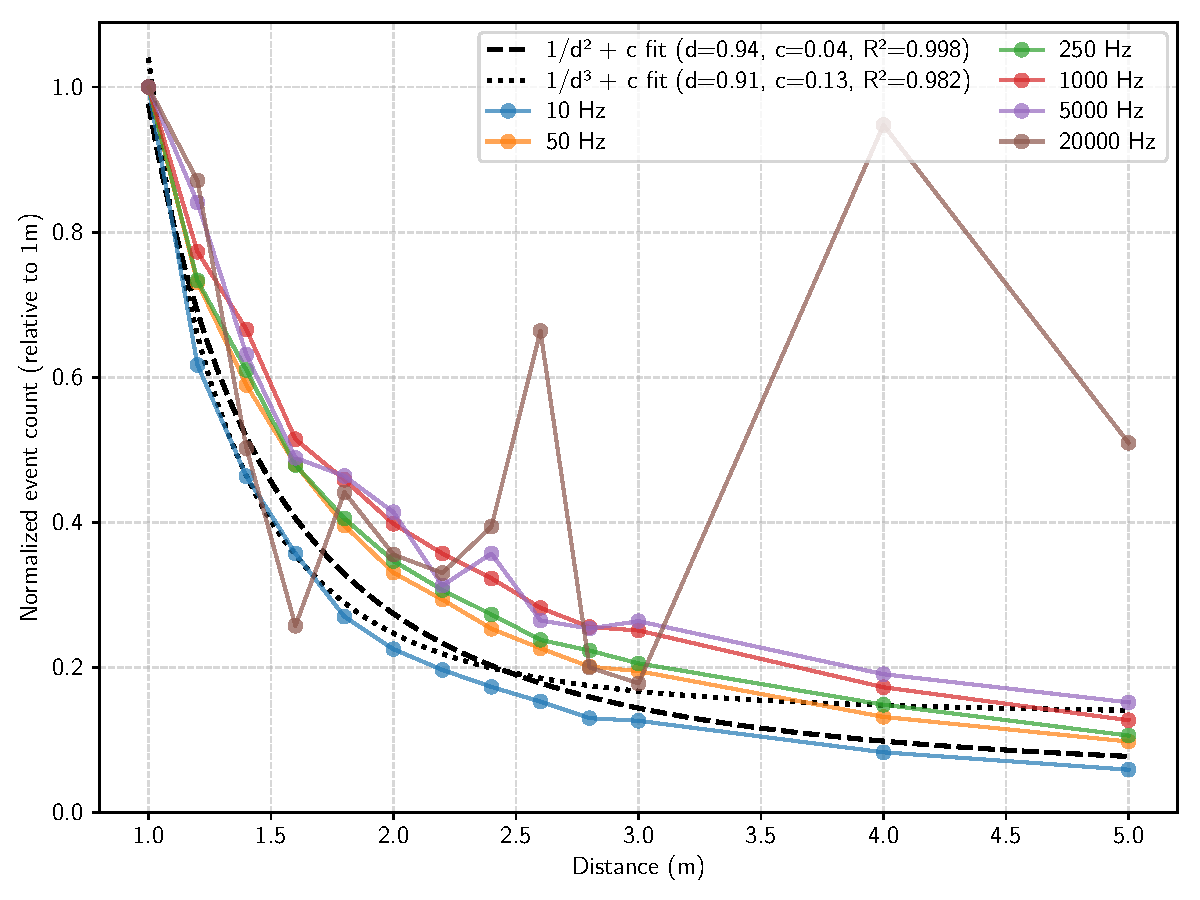
\includegraphics[width=0.50\textwidth]{../fig/pgfplot/build/inv_square.pdf}
			\caption{Experimental validation of the inverse square law}
			\label{fig:fit1}
		\end{figure}

	\end{frame}

	\begin{frame}{Perspective-n-Point}
		%describe PnP

	\end{frame}

	\begin{frame}{PnP}
		%describe PnP

	\end{frame}

	\begin{frame}[shrink=20]
		\frametitle{References}
		%\nocite{*}
		\begingroup
		\tiny
		\printbibliography[heading=none]
		\endgroup

		%The source code can be found at:
		
		%\url{https://github.com/kubakubakuba/mrs-uvdar-distance-estimator}.
	\end{frame}

\end{document}